%----------------------------------------------------------------------------------------
%	LATEX TECHNISCH RAPPORT TEMPLATE
%	Versie 1.1 (4 februari 2015)
%	Opmerkingen of feedback naar Robert van Wijk
%					(robertvanwijk@uva.nl)
%----------------------------------------------------------------------------------------

%----------------------------------------------------------------------------------------
%	PACKAGES EN DOCUMENT CONFIGURATIE
%----------------------------------------------------------------------------------------

\documentclass[a4paper,12pt]{article}
\usepackage{graphicx}
\usepackage[dutch]{babel}
\usepackage{fancyhdr}
\usepackage{lastpage}
\usepackage{xifthen}
\usepackage{algorithm2e}
\usepackage{hyperref}

%----------------------------------------------------------------------------------------
%	HEADER & FOOTER
%----------------------------------------------------------------------------------------
\pagestyle{fancy}
  \lhead{
\includegraphics[width=7cm]{logoUvA}}		%Zorg dat het logo in dezelfde map staat
  \rhead{\footnotesize \textsc {Technisch rapport\\ \opdracht}}
  \lfoot
    {
	\footnotesize \studentA
	\ifthenelse{\isundefined{\studentB}}{}{\\ \studentB}
	\ifthenelse{\isundefined{\studentC}}{}{\\ \studentC}
	\ifthenelse{\isundefined{\studentD}}{}{\\ \studentD}
	\ifthenelse{\isundefined{\studentE}}{}{\\ \studentE}
    }
  \cfoot{}
  \rfoot{\small \textsc {Pagina \thepage\ van \pageref{LastPage}}}
  \renewcommand{\footrulewidth}{0.5pt}

\fancypagestyle{firststyle}
 {
  \fancyhf{}
   \renewcommand{\headrulewidth}{0pt}
   \chead{
\includegraphics[width=7cm]{logoUvA}}
   \rfoot{\small \textsc {Pagina \thepage\ van \pageref{LastPage}}}
 }

\setlength{\topmargin}{-0.3in}
\setlength{\textheight}{630pt}
\setlength{\headsep}{40pt}

%----------------------------------------------------------------------------------------
%	DOCUMENT INFORMATIE
%----------------------------------------------------------------------------------------
%Geef bij ieder command het juiste argument voor deze opdracht. Vul het hier in en het komt op meerdere plekken in het document correct te staan.

\newcommand{\titel}{Auto Complete}			%Zelfbedachte titel
\newcommand{\opdracht}{Technisch rapport}			%Naam van opdracht die je van docent gehad hebt
\newcommand{\docent}{Floris Kroon}		%Liefst de naam van diegene die het beoordeeld
\newcommand{\cursus}{Datastructuren}
\newcommand{\vakcode}{5062DATA6Y}			%Te vinden op oa Datanose
\newcommand{\datum}{\today}					%Pas aan als je niet de datum van vanaag wilt hebben
\newcommand{\studentA}{Tijmen Zwaan}
\newcommand{\uvanetidA}{10208917}
%\newcommand{\studentB}{Naam student 2}			%Uncomment de regel als je met twee studenten werkt
\newcommand{\uvanetidB}{UvAnetID student 2}
%\newcommand{\studentC}{Naam student 3}		%Uncomment de regel als je met drie studenten werkt
\newcommand{\uvanetidC}{UvAnetID student 3}
%\newcommand{\studentD}{Naam student 4}		%Uncomment de regel als je met vier studenten werkt
\newcommand{\uvanetidD}{UvAnetID student 4}
%\newcommand{\studentE}{Naam student 5}			%Uncomment de regel als je met vijf studenten werkt
\newcommand{\uvanetidE}{UvAnetID student 5}

%----------------------------------------------------------------------------------------
%	AUTOMATISCHE TITEL
%----------------------------------------------------------------------------------------
\begin{document}
\thispagestyle{firststyle}
\begin{center}
	\textsc{\Large \opdracht}\\[0.2cm]
		\rule{\linewidth}{0.5pt} \\[0.4cm]
			{ \huge \bfseries \titel}
		\rule{\linewidth}{0.5pt} \\[0.2cm]
	{\large \datum  \\[0.4cm]}

	\begin{minipage}{0.4\textwidth}
		\begin{flushleft}
			\emph{Student:}\\
			{\studentA \\ {\small \uvanetidA \\[0.2cm]}}
				\ifthenelse{\isundefined{\studentB}}{}{\studentB \\ {\small \uvanetidB \\[0.2cm]}}
				\ifthenelse{\isundefined{\studentC}}{}{\studentC \\ {\small \uvanetidC \\[0.2cm]}}
				\ifthenelse{\isundefined{\studentD}}{}{\studentD \\ {\small \uvanetidD \\[0.2cm]}}
				\ifthenelse{\isundefined{\studentE}}{}{\studentE \\ {\small \uvanetidE \\[0.2cm]}}
		\end{flushleft}
	\end{minipage}
~
	\begin{minipage}{0.4\textwidth}
		\begin{flushright}
			\emph{Docent:} \\
			\docent \\[0.2cm]
			\emph{Cursus:} \\
			\cursus \\[0.2cm]
			\emph{Vakcode:} \\
			\vakcode \\[0.2cm]
		\end{flushright}
	\end{minipage}\\[1 cm]
\end{center}

%----------------------------------------------------------------------------------------
%	INHOUDSOPGAVE EN ABSTRACT
%----------------------------------------------------------------------------------------
%Niet doen bij korte rapporten

%\tableofcontents
%\begin{abstract}
%\lorem[13]
%\end{abstract}

%----------------------------------------------------------------------------------------
%	INTRODUCTIE
%----------------------------------------------------------------------------------------

\section{Introductie}
Het doel van deze opdracht is om een automatische aanvulfunctie te maken voor
woorden, gebaseerd op een woordenboek dat wordt opgebouwd uit een
gespecificeerde tekst. Het moet daarbij ook mogelijk zijn om woorden uit het
woordenboek te verwijderen. Het de bedoeling dat een trie-datastructuur
gebruikt wordt.

\subsection{Definities}
\begin{itemize}
    \item Node - Een punt in een netwerk of diagram waar lijnen of paden
        kruisen of splitsen.
    \item Edge - De connectie tussen twee nodes.
    \item Child - Een node die een extensie is van een andere node.
    \item Parent - De tegenovergestelde relatie als een child node.
    \item Recursief proces - Een zichzelf herhalend proces.
    \item Sequentieel proces - Een proces dat een aantal stappen doorloopt in
        een vaste volgorde.
\end{itemize}
%\subsection{Vraagstelling}

%----------------------------------------------------------------------------------------
%	METHODE
%----------------------------------------------------------------------------------------

\section{Methode}
De `trie' datastructuur lijkt op een normale `tree' datastructuur. Echter wordt
er geen data in de nodes opgeslagen, maar in de edges van de trie. Zo zullen
alle woorden beginnend met dezelfde letter de children zijn van slechts \'e\'en
node. De edge van die node heeft daarbij de waarde van de letter, en de node
bevat alleen nieuwe edges naar de volgende letters van de verschillende
woorden.

\subsection{Algoritme}
Omdat iedere node in de trie zich hetzelfde gedraagt als zowel zijn children
als zijn parents zijn veel delen goed aan te pakken op een recursieve manier.
Omdat echter na testen bleek dat een sequentiele aanpak efficienter was voor
het toevoegen van woorden is dit dus niet overal het geval.

Bij het toevoegen van een woord wordt eerst de start-node de actieve node. Er
wordt dan gekeken naar de eerste letter van het woord. Als deze al bestaat als
edge in de actieve node, wordt die node de nieuwe actieve node en gaat het
algoritme door naar de volgende letter. Als deze nog niet bestaat, wordt de
node aangemaakt en toegevoegd aan de actieve node. Daarna wordt de nieuw
aangemaakte node de actieve node.\\
Wanneer het eind van het woord bereikt is wordt in de actieve node de
zogenaamde `end-flag' op `true' gezet. Wanneer later door de trie wordt gegaan
zijn alle nodes waar deze `end-flag' op `true' staan woorden.

Binnen elke node bestaat er een lijst met de karakters die zijn toegevoegd als
children van de node. Daarnaast is er ook een lijst met de bijbehorende
child-nodes. Deze lijsten staan in dezelfde volgorde. Wanneer een specifiek
child wordt gezocht, wordt er gezocht in de eerste lijst van karakters.
Wanneer het juiste karakter is gevonden weet het programma dus ook op welke
plek de node in de andere array staat.\\
Deze arrays worden vergroot wanneer ze vol zijn, en er moet een nieuw element
bij.


%\subsection{Diagram}
%\subsection{Procedure}
%\subsection{Software en apparatuur}

\pagebreak

%----------------------------------------------------------------------------------------
%	RESULTATEN
%----------------------------------------------------------------------------------------

\section{Resultaten}

Om te testen hoe efficient dit algoritme is, heb ik het programma op teksten
van verschillende groottes losgelaten. Uit de grafiek hieronder is duidelijk
zichtbaar dat de tijd dat het programma bezig is lineair evenredig is aan het
aantal woorden in de input.\\
Als hier een zogenaamde linked-list datastructuur was gebruikt zoals in de
vorige opgave, was dit exponentieel gebleken. Dit komt doordat bij een
linked-list iedere keer door alle woorden gelopen moet worden tot het juiste
woord is bereikt. Bij de trie structuur hangt de tijd per woord af van het
aantal letters in het woord, niet van het aantal voorgaande woorden.\\

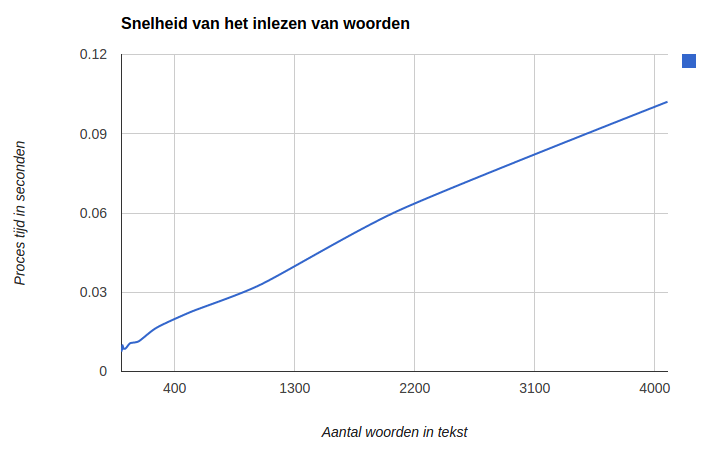
\includegraphics[width=11cm]{grafiek}


%----------------------------------------------------------------------------------------
%	DISCUSSIE
%----------------------------------------------------------------------------------------

\section{Discussie}

In mijn eerste implementatie van dit probleem had ik besloten om in iedere node
een array van 26 pointers neer te zetten. E\'en pointer voor iedere letter
van het alphabet. Hierdoor is een pointer `NULL' wanneer de edge niet bestaat
en anders wijst hij naar de juiste node. Dit zorgt ervoor dat er binnen een
node niet gezocht hoeft te worden naar de edges. Echter limiteert dit het
woordenboek tot slechts 26 tekens. Dit is in de huidige implementatie niet zo
wat betekent dat alle karakters toegevoegd kunnen worden, maar er dus wel
extra tijd nodig is om binnen een node te zoeken naar de correcte child-node.

%\subsection{Implicaties en aanbevelingen}
%\subsection{Conclusie}


%----------------------------------------------------------------------------------------
%	REFERENTIES
%----------------------------------------------------------------------------------------
%Meer informatie hierover volgt in blok 5 van jaar 1.

\bibliographystyle{acm}

%----------------------------------------------------------------------------------------
%	BIJLAGEN
%----------------------------------------------------------------------------------------

%\section{Bijlage A}
%\section{Bijlage B}
%\section{Bijlage C}

\end{document}
